\section*{Introduction}
Dans ce chapitre, nous présenterons le corpus, les expérimentations et les différents choix effectués pour les tests.
\section{Corpus}
Différence de qualité de jeu\\
\textbf{groove MIDI dataset}\\
\url{https://magenta.tensorflow.org/datasets/groove}\\\\
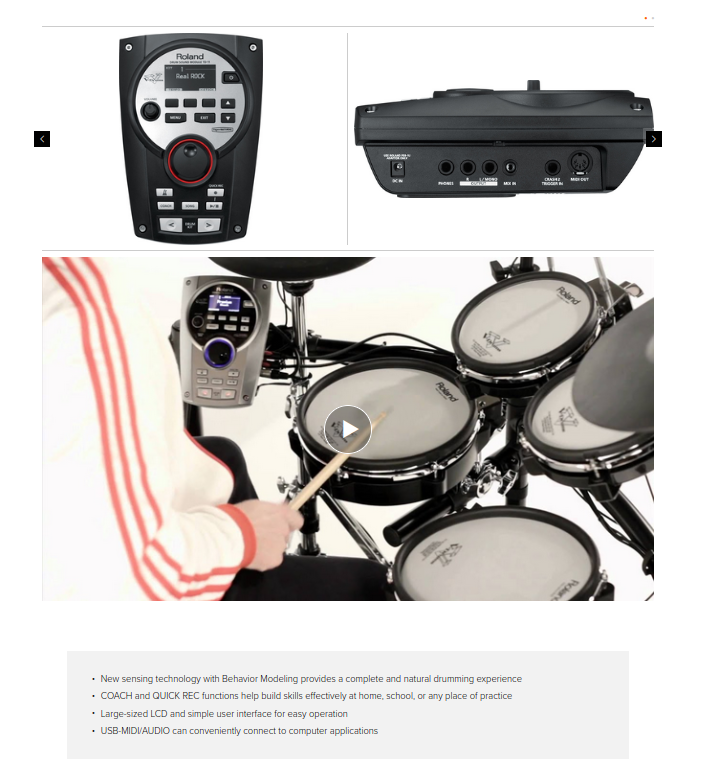
\includegraphics[height=60mm, width=60mm]{z_images/3_groove/roland_TD11.png}\\
Des batteurs pro ont été engagés pour jouer sur un roland td-11\\\\
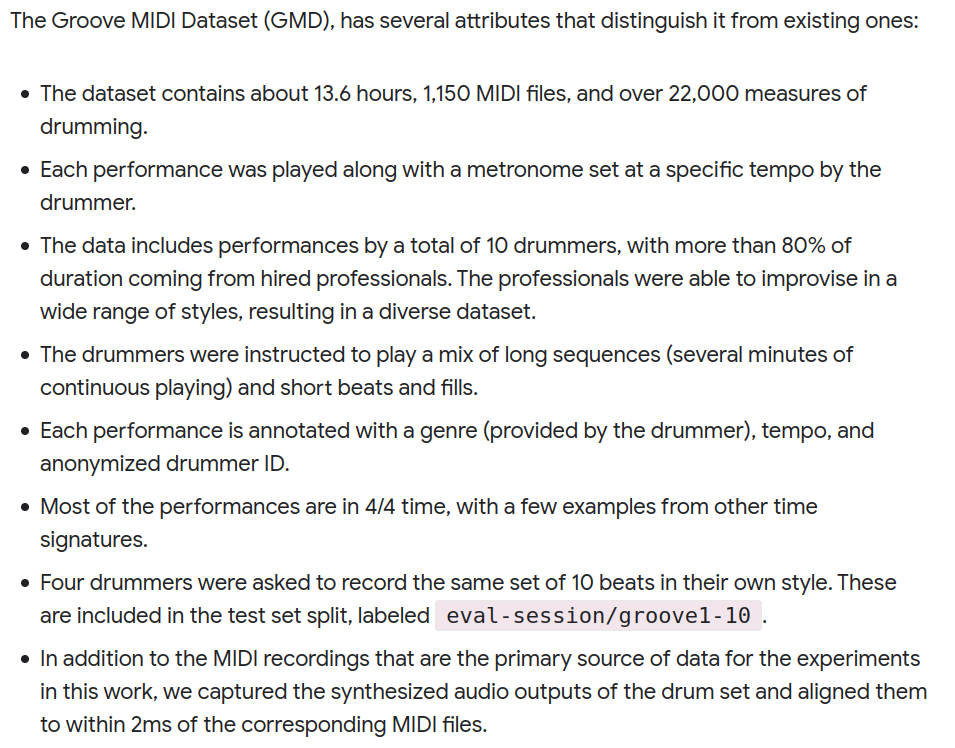
\includegraphics[height=80mm, width=110mm]{z_images/3_groove/dataset_how.png}\newpage{}
\textbf{Les métadatas :}\\\\
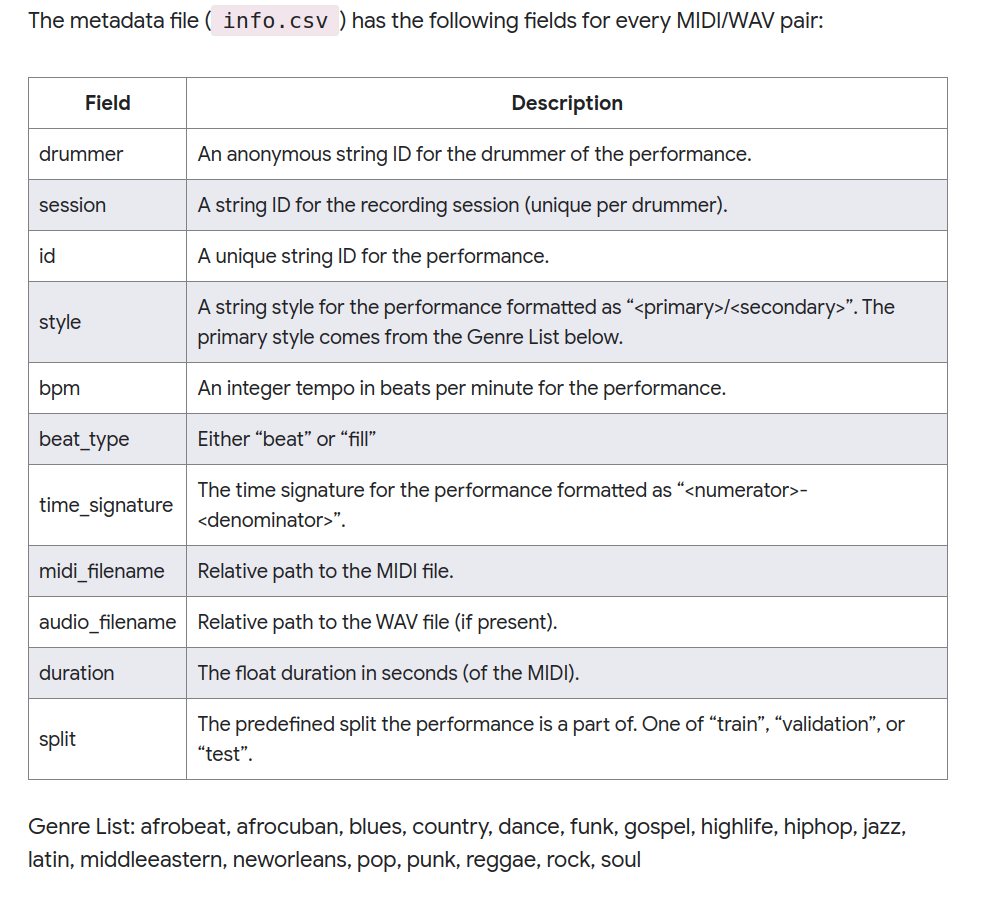
\includegraphics[height=85mm, 
width=100mm]{z_images/3_groove/csv_metadata_struct.png}\\
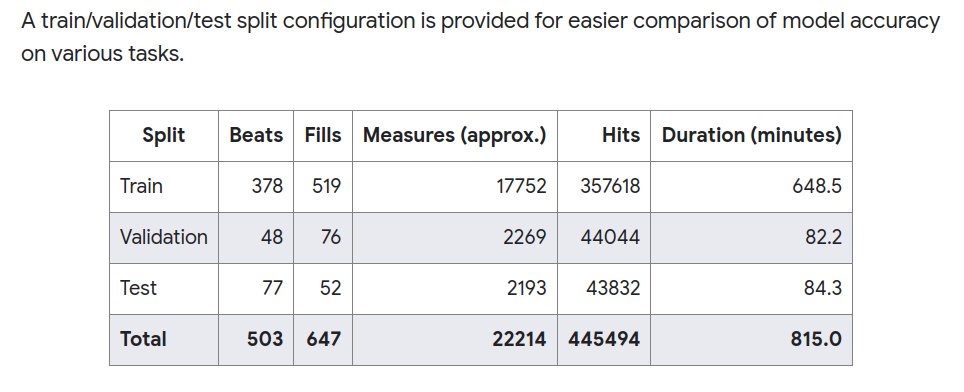
\includegraphics[height=50mm, width=120mm]{z_images/3_groove/train_validation_test.png}\\
Détails (entre autres tensorflow avec le dataset) à :
\url{https://magenta.tensorflow.org/datasets/groove#license}\\
écouter le dataset groove
\section{Analyse MIDI-Audio}
\label{analyse_midi_audio}
Ces analyses ont été faites essentiellement dans le cadre de transcription manuelles à partir de fichiers MIDI et Audio du Groove MIDI Data Set. Les partitions manuelles sont éditées à l’aide de lilypond\footnote{\url{http://lilypond.org/}}. Les transcriptions automatiques sont générées avec MuseScore\footnote{\url{https://musescore.com/}}.
\subsection{Comparaisons de transcriptions}
Transcription manuelle VS transcription automatique :\\
\textit{drummer\_01/session3 — 10\_rock-folk\_90\_beat\_4-4}\\\\
Fichier midi vers partition avec musescore $\Rightarrow$ Transcription manuelle\\
\includegraphics[height=20mm, width=50mm]{z_images/transcriptions_manuelles/0_prise_en_main/0_tests_drummer_01__session3/musescore_0.png}\ \ \ \ 
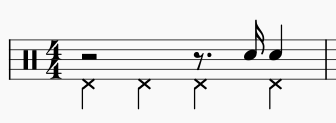
\includegraphics[height=20mm, width=55mm]{z_images/transcriptions_manuelles/0_prise_en_main/0_tests_drummer_01__session3/manuel_0.png}
\textit{drummer\_01/session3 — 10\_rock-folk\_90\_beat\_4-4}\\\\
Fichier midi vers partition avec musescore $\Rightarrow$ Transcription manuelle\\
\includegraphics[height=20mm, width=50mm]{z_images/transcriptions_manuelles/0_prise_en_main/0_tests_drummer_01__session3/musescore_0.png}\ \ \ \ 
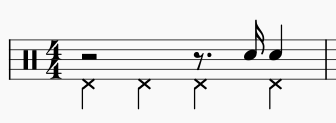
\includegraphics[height=20mm, width=55mm]{z_images/transcriptions_manuelles/0_prise_en_main/0_tests_drummer_01__session3/manuel_0.png}
\begin{itemize}
	\item Erreur d’indication de mesure ;
	\item Mauvaise transcription d’une noire.\\
\end{itemize}
La noire du 4ème temps se retrouve sur le premier temps de la mesure suivante et elle se transforme en un triolet de double croches dont seules les deux premières seraient jouées.\\\\
\textit{drummer\_01/session3 — 10\_rock-folk\_90\_beat\_4-4}\\\\
Fichier midi vers partition avec musescore $\Rightarrow$ Transcription manuelle\\
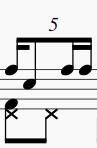
\includegraphics[height=20mm, width=15mm]{z_images/transcriptions_manuelles/0_prise_en_main/0_tests_drummer_01__session3/musescore_1.png}\ \ \ \ 
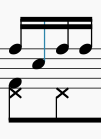
\includegraphics[height=20mm, width=15mm]{z_images/transcriptions_manuelles/0_prise_en_main/0_tests_drummer_01__session3/manuel_1.png}\\
\begin{itemize}
	\item Erreur de quantification : les doubles croches ont été interprétées en quintolet;\\
\end{itemize}
drummer\_01/session3 — 2\_jazz-swing\_185\_beat\_4-4\\\\
Fichier midi vers partition avec musescore $\Rightarrow$ Transcription manuelle\\
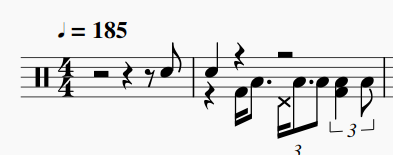
\includegraphics[height=25mm, width=60mm]{z_images/transcriptions_manuelles/0_prise_en_main/0_tests_drummer_01__session3/musescore_2.png}\ \ \ \ 
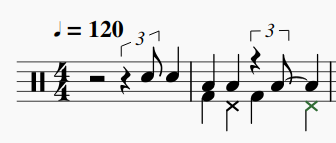
\includegraphics[height=25mm, width=55mm]{z_images/transcriptions_manuelles/0_prise_en_main/0_tests_drummer_01__session3/manuel_2.png}
\begin{itemize}
	\item L’indication de mesure est correcte mais tout a été décalé d’un temps car la première noire sur la caisse claire est jouée sur le 4ème temps et non sur le premier temps de la deuxième mesure comme l’indique la transcription de musescore.
	\item Les toms basses des 1er et 2ème temps de la mesure musescore auraient dû être sur les temps et non décalés d’une double croche vers la droite.\\
\end{itemize}
drummer\_01/session1 — 1\_funk\_80\_beat\_4-4\\\\
Fichier midi vers partition avec musescore $\Rightarrow$ Transcription manuelle\\
\includegraphics[height=25mm, width=40mm]{z_images/transcriptions_manuelles/0_prise_en_main/1_drummer_01__session1/musescore_0.png}\ \ \ \ 
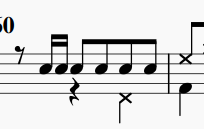
\includegraphics[height=25mm, width=40mm]{z_images/transcriptions_manuelles/0_prise_en_main/1_drummer_01__session1/Manuelle_0.png}
\begin{itemize}
	\item On dirait que lorsque certaines notes sont proches, elles se resserrent et suppriment celles qui aurait dû être sur le temps.\\
	\item Erreur d’indication de mesure ;
	\item Mauvaise transcription d’une noire.\\
\end{itemize}
La noire du 4ème temps se retrouve sur le premier temps de la mesure suivante et elle se transforme en un triolet de double croches dont seules les deux premières seraient jouées.\\\\
\textit{drummer\_01/session3 — 10\_rock-folk\_90\_beat\_4-4}\\\\
Fichier midi vers partition avec musescore $\Rightarrow$ Transcription manuelle\\
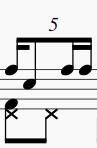
\includegraphics[height=20mm, width=15mm]{z_images/transcriptions_manuelles/0_prise_en_main/0_tests_drummer_01__session3/musescore_1.png}\ \ \ \ 
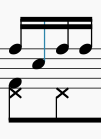
\includegraphics[height=20mm, width=15mm]{z_images/transcriptions_manuelles/0_prise_en_main/0_tests_drummer_01__session3/manuel_1.png}\\
\begin{itemize}
	\item Erreur de quantification : les doubles croches ont été interprétées en quintolet;\\
\end{itemize}
drummer\_01/session3 — 2\_jazz-swing\_185\_beat\_4-4\\\\
Fichier midi vers partition avec musescore $\Rightarrow$ Transcription manuelle\\
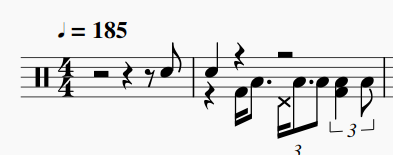
\includegraphics[height=25mm, width=60mm]{z_images/transcriptions_manuelles/0_prise_en_main/0_tests_drummer_01__session3/musescore_2.png}\ \ \ \ 
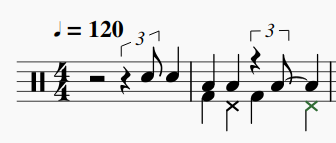
\includegraphics[height=25mm, width=55mm]{z_images/transcriptions_manuelles/0_prise_en_main/0_tests_drummer_01__session3/manuel_2.png}
\begin{itemize}
	\item L’indication de mesure est correcte mais tout a été décalé d’un temps car la première noire sur la caisse claire est jouée sur le 4ème temps et non sur le premier temps de la deuxième mesure comme l’indique la transcription de musescore.
	\item Les toms basses des 1er et 2ème temps de la mesure musescore auraient dû être sur les temps et non décalés d’une double croche vers la droite.\\
\end{itemize}
drummer\_01/session1 — 1\_funk\_80\_beat\_4-4\\\\
Fichier midi vers partition avec musescore $\Rightarrow$ Transcription manuelle\\
\includegraphics[height=25mm, width=40mm]{z_images/transcriptions_manuelles/0_prise_en_main/1_drummer_01__session1/musescore_0.png}\ \ \ \ 
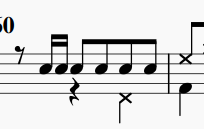
\includegraphics[height=25mm, width=40mm]{z_images/transcriptions_manuelles/0_prise_en_main/1_drummer_01__session1/Manuelle_0.png}
\begin{itemize}
	\item On dirait que lorsque certaines notes sont proches, elles se resserrent et suppriment celles qui aurait dû être sur le temps.\\
\end{itemize}
\textbf{Exemple avec des flas}\\\\
Fichier midi vers partition avec musescore :\\
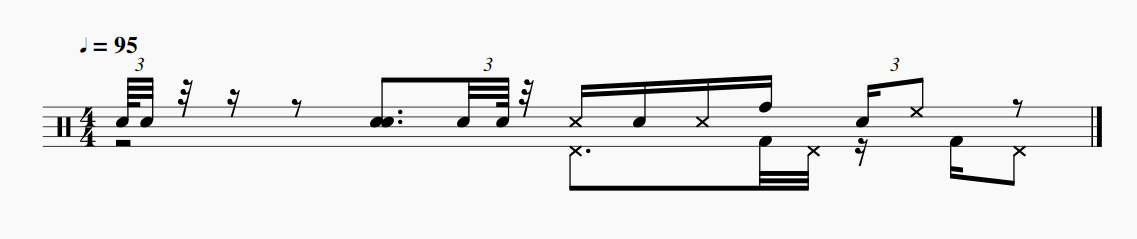
\includegraphics[height=30mm, width=120mm]{z_images/transcriptions_manuelles/1_transcriptions_flas/124_funk_95_fill_4-4_0.png}\\
Transcription manuelle :\\
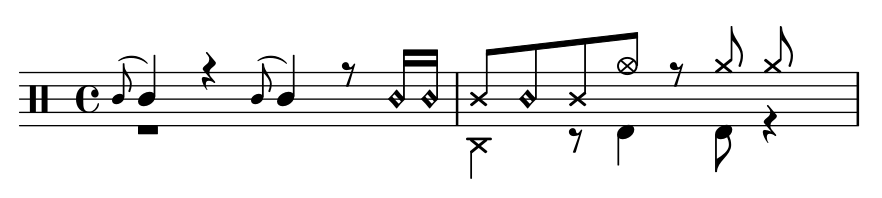
\includegraphics[height=20mm, width=90mm]{z_images/transcriptions_manuelles/1_transcriptions_flas/124_funk_95_fill_4-4_1_.png}\\
MuseScore donne un aperçu de l’état de l’art pour la transcription de la batterie.
\newpage
\subsection{Transcription de partition}
\begin{figure}[h]
	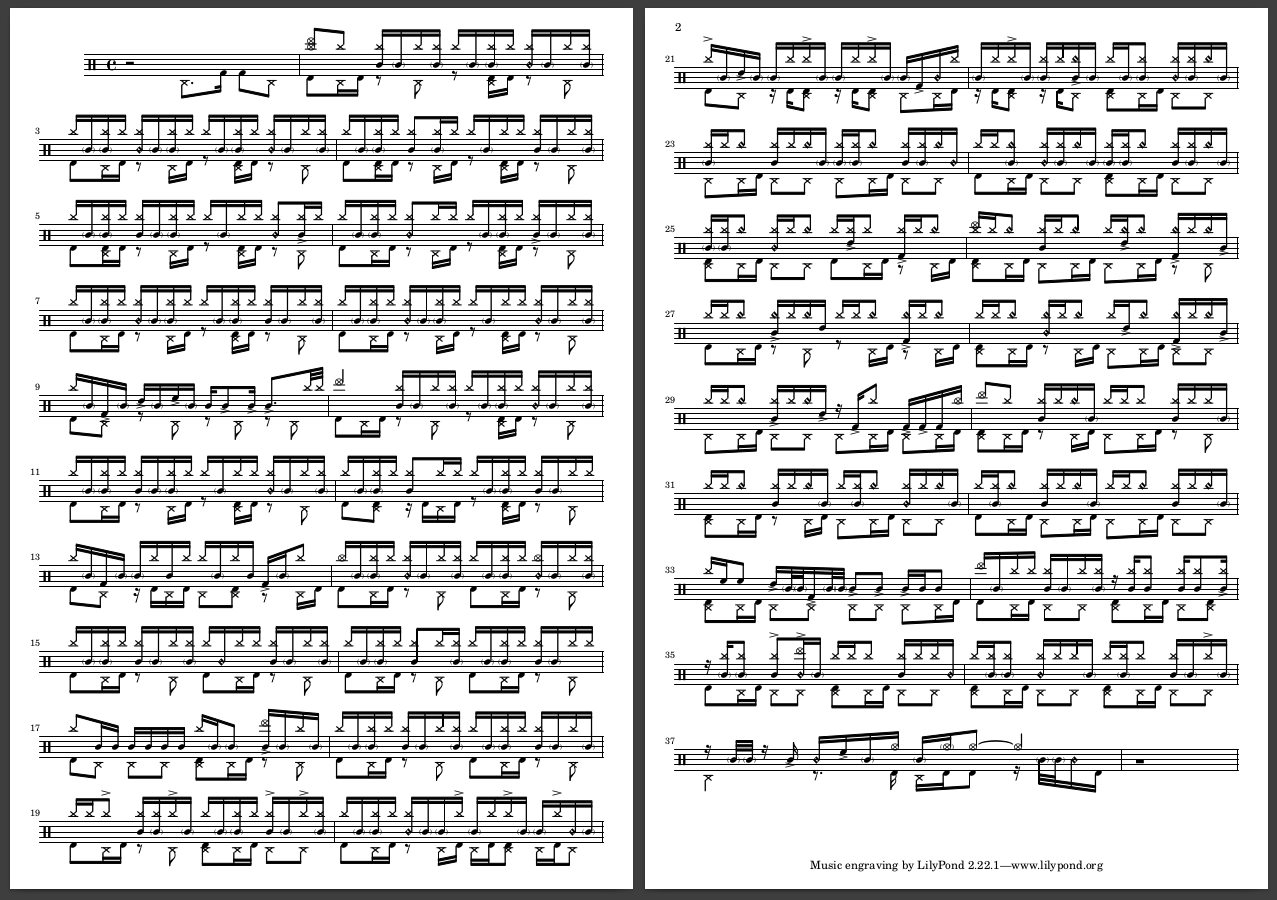
\includegraphics[height=120mm, width=160mm]{z_images/4_experimentations/experience_1/partition.png}
	\caption{référence 1}
\end{figure}
Il s’agit d’une partition d’un 4/4 binaire dont le fichier MIDI est annoncé dans le groove-dataset de style «jazz-funk» probablement en raison de la ride de type shabada rapide (le ternaire devient binaire avec la vitesse) combiné avec l’after-beat de type rock (caisse-claire sur les deux et quatre).\\
La transcription de cette partition a occasionné plusieurs remarque :\\
- vélocité, place des accents, etc…
\section{Expérimentation théorique d’un système}
\subsection{Motifs}
\begin{figure}[h]
	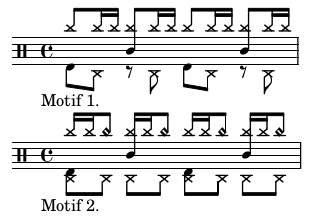
\includegraphics[height=30mm, width=40mm]{z_images/description_notation/systemes/1_motifs_4-4_binaires.png}
	\caption{Motifs}
\end{figure}
Les motifs 1 et 2 peuvent être extraits de la figure 3.8. Ces deux motifs sont très classiques et seront réutilisables aussi dans d’autres contextes.\\
Le motif 1 est joué jusqu’à la mesure 18 avec des variations et des breaks.\\
Le motif 2 est joué des mesures 23 à 28.\\\\
\subsection{Gammes}
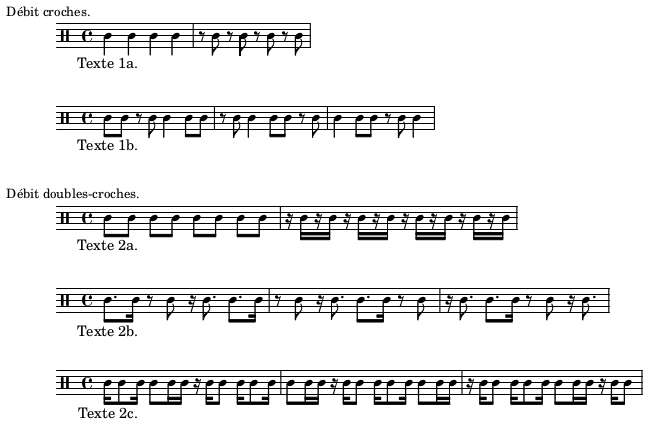
\includegraphics[height=70mm, width=95mm]{z_images/description_notation/systemes/0_textes_4-4_binaires.png}\\

\subsection{Systèmes}
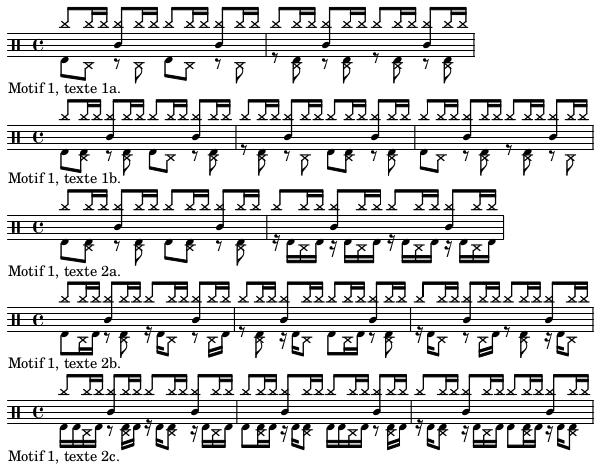
\includegraphics[height=75mm, width=85mm]{z_images/4_experimentations/experience_1/systeme_recherche_1.png}
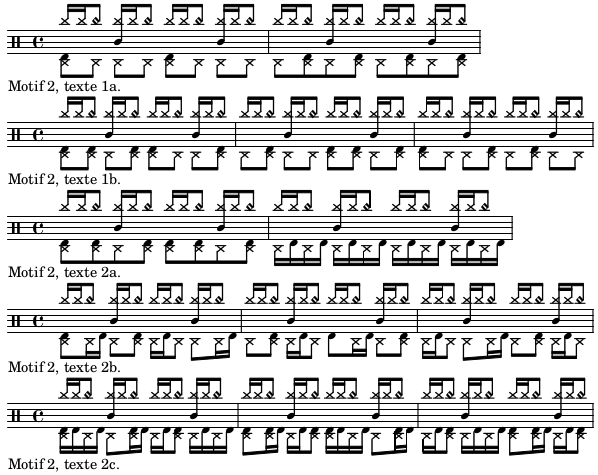
\includegraphics[height=75mm, width=85mm]{z_images/4_experimentations/experience_1/systeme_recherche_2.png}
\newpage

\subsection{Démonstration}
\textbf{Représentation des systèmes en arbres de rythmes}

\resizebox{440pt}{!} {
	\Tree[.Motif\ 1\ +\ Texte\ 1a
	[.Mesure\ 1
	[.Temps\ 1 [rd\\bd ][ [rd\\pf ][rd ]]]
	[.Temps\ 2 [rd\\cc ][ [rd\\pf ][rd ]]]
	[.Temps\ 3 [rd\\bd ][ [rd\\pf ][rd ]]]
	[.Temps\ 4 [rd\\cc ][ [rd\\pf ][rd ]]] ]
	[.Mesure\ 2
	[.Temps\ 1 [rd ][ [rd\\bd\\pf ][rd ]]]
	[.Temps\ 2 [rd\\cc ][ [rd\\bd\\pf ][rd ]]]
	[.Temps\ 3 [rd ][ [rd\\bd\\pf ][rd ]]]
	[.Temps\ 4 [rd\\cc ][ [rd\\bd\\pf ][rd ]]] ]]}
\textbf{Réécriture}
\textit{Règles établies par le système}\\
\textbf{Séparation des voix}\\
\textit{Voix haute}\\
\resizebox{440pt}{!} {
	\Tree[.Motif\ 1\ +\ Texte\ 1a
	[.Mesure\ 1
	[.Temps\ 1 [rd ][ [rd ][rd ]]]
	[.Temps\ 2 [rd\\cc ][ [rd ][rd ]]]
	[.Temps\ 3 [rd ][ [rd ][rd ]]]
	[.Temps\ 4 [rd\\cc ][ [rd ][rd ]]] ]
	[.Mesure\ 2
	[.Temps\ 1 [rd ][ [rd ][rd ]]]
	[.Temps\ 2 [rd\\cc ][ [rd ][rd ]]]
	[.Temps\ 3 [rd ][ [rd ][rd ]]]
	[.Temps\ 4 [rd\\cc ][ [rd ][rd ]]] ]]}\\

\textit{Voix basse}\\
\resizebox{440pt}{!} {
	\Tree[.Motif\ 1\ +\ Texte\ 1a
	[.Mesure\ 1
	[.Temps\ 1 [bd ][ [pf ][t ]]]
	[.Temps\ 2 [t ][ [pf ][t ]]]
	[.Temps\ 3 [bd ][ [pf ][t ]]]
	[.Temps\ 4 [t ][ [pf ][t ]]] ]
	[.Mesure\ 2
	[.Temps\ 1 [t ][ [bd\\pf ][t ]]]
	[.Temps\ 2 [t ][ [bd\\pf ][t ]]]
	[.Temps\ 3 [t ][ [bd\\pf ][t ]]]
	[.Temps\ 4 [t ][ [bd\\pf ][t ]]] ]]}\\

\textbf{Règles de simplifications pour le 4/4 binaire}\\
Simplifier l’écriture de chaque voix (\textit{Règles établis par le système})\\
\resizebox{70pt}{!} {
	\Tree[.1/4 [t ][x ][x ][x ] ]
}\ \ \ \ \ $\Rightarrow$\ \ \ \ \
\resizebox{70pt}{!} {
	\Tree[.1/4 [r ][x ][x ][x ] ]
}\\\\

\resizebox{70pt}{!} {
	\Tree[.1/4 [x ][t ][x ][x ]]
}\ \ \ \ \ $\Rightarrow$\ \ \ \ \
\resizebox{50pt}{!} {
	\Tree[.1/4 [x ][ [x ][x ]]]
}\\\\

\resizebox{70pt}{!} {
	\Tree[.1/4 [t ][x ][x ][t ] ]
}\ \ \ \ \ $\Rightarrow$\ \ \ \ \
\resizebox{50pt}{!} {
	\Tree[.1/4 [ [r ][x ]][x ] ]
}\\\\

\resizebox{50pt}{!} {
	\Tree[.1/4 [t ][ [x ][x ]]]
}\ \ \ \ \ $\Rightarrow$\ \ \ \ \
\resizebox{50pt}{!} {
	\Tree[.1/4 [r ][ [x ][x ]]]
}\\\\

\resizebox{50pt}{!} {
	\Tree[.1/4 [t ][ [x ][t ]] ]
}\ \ \ \ \ $\Rightarrow$\ \ \ \ \
\resizebox{30pt}{!} {
	\Tree[.1/4 [r ][x ] ]
}\\\\

\resizebox{50pt}{!} {
	\Tree[.1/4 [x ][ [x ][t ]] ]
}\ \ \ \ \ $\Rightarrow$\ \ \ \ \
\resizebox{30pt}{!} {
	\Tree[.1/4 [x ][x ] ]
}
\section{Développement}
\subsection{DrumCode}
Adaptation de la modélisation pour la transcription en cpp.
\subsection{Tests unitaires sur les Jams}
\label{jam_tests}
Les Jams permettent de passer du monophonique au polyphonique.
\subsection{Parsing}
\label{gram_pond}
Tests effectués avec le fichier midi suivant :\\\\
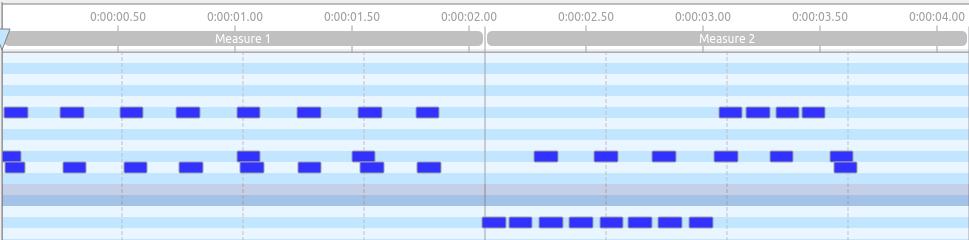
\includegraphics[height=50mm, width=160mm]{z_images/4_experimentations/input_parsing/midi_2bars_fill.png}\\\\
%\textit{Voix basse}\\
Un premier test convaincant est effectué avec la grammaire suivante :\\\\
// bar level\\
0 -> C0                1\\
0 -> E1                1\\
0 -> U4(1, 1, 1, 1)    1\\

// half bar level\\
9 -> C0                1\\
9 -> E1                1\\

// beat level\\
1 -> C0                1\\
1 -> E1                1\\
1 -> T2(2, 2)          1\\
1 -> T4(4, 4, 4, 4)    1\\

// croche level\\
2 -> C0                1\\
2 -> E1                1\\

// double level\\
4 -> C0                1\\
4 -> E1                1\\
4 -> E2                1\\
4 -> T2(6, 6)          1\\

// triple level\\
6 -> E1                1\\\\
Cette grammaire sépare les ligatures par temps au niveau de la mesure. Puis, au niveau du temps, elle autorise les divisions par deux (croches) et par quatre (doubles-croches). Tous les poids sont réglés sur 1. L’arbre de parsing en résultant est considéré comme « convaincant » car il découpe correctement les mesures et les temps.
\\\\
\resizebox{450pt}{!} {
\Tree[.Mesure\ 1
[.Temps\ 1 [0-ON\\1-ON\\2-ON ][3-OFF\\4-OFF\\5-OFF ][6-ON\\7-ON ][8-OFF\\9-OFF ]]
[.Temps\ 2 [10-ON\\11-ON ][12-OFF\\13-OFF ][14-ON\\15-ON ][16-OFF\\17-OFF ]]
[.Temps\ 3 [18-ON\\19-ON\\20-ON ][21-OFF\\22-OFF\\23-OFF ][24-ON\\25-ON ][26-OFF\\27-OFF ]]
[.Temps\ 4 [28-ON\\29-ON\\30-ON ][31-OFF\\32-OFF\\33-OFF ][34-ON\\35-ON ][36-OFF\\37-OFF ]]
]}\\\\\\
Les temps de la première mesure du fichier MIDI sont bien quantifié mais ceux de la deuxième mesure présentent quelques défauts de quantification visibles dès le premier temps.\\\\
\resizebox{300pt}{!} {
\Tree[.Mesure\ 2
[.Temps\ 1 [38-ON ][ [39-OFF ][40-ON ] ][ [41-OFF\\42-ON ][43-ON ] ][ [44-OFF\\45-OFF ][46-ON ] ]]
]}\\\\\\
Les Onsets sont correctement triés au niveau des doubles croches mais certaines doubles croches sont inutilement subdivisées en triples croches (les 2ème, 3ème et 4ème doubles croches sur le premier temps ci-dessus).\\\\
\textbf{2ème exemple :}\\
Après une augmentation du poids des triples croches dans la grammaire (monté de 1 à 5)et une baisse de tous les autres poids (descendu de 1 à 0.5), et mis à part le troisième temps de la 2ème mesure, tous les Onsets sont bien triés et aucuns ne sont subdivisés.






%\newpage
%\section{Résultats et discussion}
%\subsection{Résultats}
%\subsection{Évaluation}
%1 - Transcription manuelle à partir de fichier midi et/ou wav d’une partition contenant des systèmes. Écriture des systèmes contenues dans la partition (arbres, séparation des voix, réécriture)\\\\

\section*{Conclusion}
Conclusion de ce chapitre.